% !TEX TS-program = pdflatex
% !TEX encoding = UTF-8 Unicode

% This is a simple template for a LaTeX document using the "article" class.
% See "book", "report", "letter" for other types of document.

\documentclass[11pt]{article} % use larger type; default would be 10pt

\usepackage[utf8]{inputenc} % set input encoding (not needed with XeLaTeX)

%%% Examples of Article customizations
% These packages are optional, depending whether you want the features they provide.
% See the LaTeX Companion or other references for full information.

%%% PAGE DIMENSIONS
\usepackage{geometry} % to change the page dimensions
\geometry{a4paper} % or letterpaper (US) or a5paper or....
% \geometry{margins=2in} % for example, change the margins to 2 inches all round
% \geometry{landscape} % set up the page for landscape
%   read geometry.pdf for detailed page layout information

\usepackage{graphicx} % support the \includegraphics command and options

% \usepackage[parfill]{parskip} % Activate to begin paragraphs with an empty line rather than an indent

%%% PACKAGES
\usepackage{booktabs} % for much better looking tables
\usepackage{array} % for better arrays (eg matrices) in maths
\usepackage{paralist} % very flexible & customisable lists (eg. enumerate/itemize, etc.)
\usepackage{verbatim} % adds environment for commenting out blocks of text & for better verbatim
\usepackage{subfig} % make it possible to include more than one captioned figure/table in a single float
% These packages are all incorporated in the memoir class to one degree or another...

%%% HEADERS & FOOTERS
\usepackage{fancyhdr} % This should be set AFTER setting up the page geometry
\pagestyle{fancy} % options: empty , plain , fancy
\renewcommand{\headrulewidth}{0pt} % customise the layout...
\lhead{}\chead{}\rhead{}
\lfoot{}\cfoot{\thepage}\rfoot{}

%%% SECTION TITLE APPEARANCE
\usepackage{sectsty}
\allsectionsfont{\sffamily\mdseries\upshape} % (See the fntguide.pdf for font help)
% (This matches ConTeXt defaults)

%%% ToC (table of contents) APPEARANCE
\usepackage[nottoc,notlof,notlot]{tocbibind} % Put the bibliography in the ToC
\usepackage[titles,subfigure]{tocloft} % Alter the style of the Table of Contents
\renewcommand{\cftsecfont}{\rmfamily\mdseries\upshape}
\renewcommand{\cftsecpagefont}{\rmfamily\mdseries\upshape} % No bold!

%%% END Article customizations
%%%package added by Wenge
%%%\usepackage{esint}
\usepackage{amsmath}
\usepackage{graphicx}
\graphicspath{ {./images/} }
%%% The "real" document content comes below...

\title{Notes for fluid dynamics}
\author{Wenge Huang}
%\date{} % Activate to display a given date or no date (if empty),
         % otherwise the current date is printed 

\begin{document}
\maketitle

\section{Basic equation}
\subsection{Substantial derivative}
\hspace{5mm}
$\frac{D}{Dt}$ is called the substantial derivative. $\frac{D\rho}{Dt}$ is the instantaneous time rate of change of density of the fluid element as it moves through a point. Here our eyes are locked on the fluid element as it is moving, and we are watching the density change of the element as it moves through the point. \par
This is different from $\frac{\partial \rho}{\partial t}$, which is physically the time rate of change of density at the fixed point. \par
$\frac{D\rho}{Dt}$ and $\frac{\partial \rho}{\partial t}$ are physically and numerically different quantities. \par
Here we show the definition of $\frac{D}{Dt}$. If we have
$$
\rho_{1} = \rho_{1}(x_{1}, y_{1}, z_{1}, t_{1})
$$
$$
\rho_{2} = \rho_{2}(x_{2}, y_{2}, z_{2}, t_{2})
$$
Then we calculate that
\begin{equation}
\frac{D\rho}{Dt} = \lim_{t_{1} \to t_{2}}\frac{\rho_{2}-\rho_{1}}{t_{1}-t_{2}}
\end{equation}
\begin{equation}
\frac{D\rho}{Dt} = \frac{\partial \rho}{\partial t}+u\frac{\partial \rho}{\partial x}+v\frac{\partial \rho}{\partial y}+w\frac{\partial \rho}{\partial z}
\end{equation}
\begin{equation}
\frac{D}{Dt} = \frac{\partial }{\partial t}+\vec{v}\cdot \nabla
\end{equation}
The first part is the local derivative and the second part is the convective derivative.\par
The substantial derivative is essentially the total derivative from calculus. For example:
$$
d\rho = \frac{\partial \rho}{\partial t}dt+\frac{\partial \rho}{\partial x}dx+\frac{\partial \rho}{\partial y}dy+\frac{\partial \rho}{\partial z}dz
$$
$$
\frac{D\rho}{Dt} = \frac{d \rho}{d t} = \frac{\partial \rho}{\partial t}+\frac{\partial \rho}{\partial x}\frac{dx}{dt}+\frac{\partial \rho}{\partial y}\frac{dy}{dt}+\frac{\partial \rho}{\partial z}\frac{dz}{dt}
$$



\subsection{Conservation of mass}
\hspace{5mm} We consider the finite control volume (here we consider that the CV is fixed in space, which means the shape of the volume is unchanged).\par
Mass is conserved: \textbf{Net mass flow out of the control volume through surface $S$ is equal to the time rate of decrease of mass inside the control volume $V$}.\par
The mass flux across a surface element $d\vec{S}$ is:
$$
\rho\vec{v}\cdot d\vec{S}
$$
The net mass flow out of control volume is:
$$
\iint_{S}\rho\vec{v}\cdot d\vec{S}
$$
The total mass inside the control volume is:
$$
\iiint_{V} \rho dV
$$
Since we consider the fixed control volume, the time rate of increase of mass inside the CV $V$ is then:
$$
\frac{\partial}{\partial t}\iiint_{V} \rho dV
$$Note that the time rate of decrease is negative, while the net mass flux out is positive. When considering conservation, we should make the sign correct.\par
Thus we have the conservation of mass:
\begin{equation}
\frac{\partial}{\partial t}\iiint_{V} \rho dV + \iint_{S}\rho\vec{v}\cdot d\vec{S} = 0
\end{equation}\par
Now we consider the control volume moving with the fluid. The control volume is always made up of the same fluid particles as it moves with the flow. The mass is fixed, but the volume $V$ and the control surface $S$ is always changing.\par
The total mass of the finite control volume is:
$$
M = \iiint_{\Omega} \rho d\Omega
$$
The volume integral is taken over the whole moving control volume $\Omega$. But the control volume is changing as the control volume moves downstream.\par
Since the mass $M$ is constant, it doesn't change with time, mathematically:
$$
\frac{dM}{dt} = 0
$$\par
Here we use the form of the substantial derivative:
\begin{equation}
\frac{D}{Dt} \iiint_{\Omega} \rho d\Omega =0
\end{equation}
Again, we get the integral form of the continuity equation (nonconservation form). We have obtained the \textbf{integral} form of the continuity equation in two different ways. Now we are trying to get the \textbf{differential} form also in two different ways. Note that it is not a simple transfer from the integral to differential mathematically. \par
This time, we don't consider the finite control volume $V$ but an infinitesimally small element $dxdydz$ (fixed in space).\par
The Net mass flux for the infinitesimally small element in $x$ is:
$$
\left[ \rho u + \frac{\partial \rho u}{\partial x}dx\right] \cdot dydz 
-(\rho u) dydz = \frac{\partial \rho u}{\partial x}dxdydz
$$
$$
\left[ \rho v + \frac{\partial \rho v}{\partial y}dx\right] \cdot dxdz 
-(\rho v) dxdz = \frac{\partial \rho v}{\partial y}dxdydz
$$
$$
\left[ \rho w + \frac{\partial \rho w}{\partial z}dz\right] \cdot dydx 
-(\rho w) dydx = \frac{\partial \rho w}{\partial z}dxdydz
$$As a result, the total net mass flow is:
$$
\left[\frac{\partial (\rho u)}{\partial x}+\frac{\partial (\rho v)}{\partial y}+ \frac{\partial (\rho w)}{\partial z}\right]dxdydz
$$\par
The time rate of mass is:
$$
\frac{\partial \rho}{\partial t}dxdydz
$$\par
Finally, we get the differential form of the continuity equation:
\begin{equation}
\frac{\partial \rho}{\partial t} +\frac{\partial (\rho u)}{\partial x}+\frac{\partial (\rho v)}{\partial y}+ \frac{\partial (\rho w)}{\partial z} = 0
\end{equation}
$$
\frac{\partial \rho}{\partial t} +\nabla \cdot(\rho \vec{v})=0
$$\par
The moving control volume mode. The mass of the infinitesimally small fluid element is:
$$
\delta m = \rho \delta \Omega
$$
Since the mass is conserved, we have:
$$
\frac{D (\delta m)}{Dt} = \frac{D (\rho \delta \Omega)}{Dt}= 0
$$
The derivative by part allows us to get:
$$
\frac{D \rho}{Dt} + \frac{\rho}{\delta \Omega}\cdot\frac{D ( \delta \Omega)}{Dt}= 0
$$\par
The volume can be calculated as:
$$
\delta \Omega = \iint_{\delta S}\vec{v}dS \cdot \delta t
$$
$$
\frac{D ( \delta \Omega)}{Dt} =\lim_{\delta t \to 0} \frac{\delta \Omega}{\delta t}=\lim_{\delta s \to 0}\iint_{\delta S}\vec{v}dS =\lim_{\delta \Omega \to 0}\iiint_{\delta \Omega} (\nabla \cdot \vec{v})d \Omega = (\nabla \cdot \vec{v})\delta \Omega
$$\par
As a result, we find another form of the continuity equation:
\begin{equation}
\frac{D \rho}{Dt} + \rho  (\nabla \cdot \vec{v})= 0
\end{equation}
Note that
$$
\frac{D \rho}{Dt} + \rho  (\nabla \cdot \vec{v}) = \frac{\partial \rho}{\partial t} + \vec{v} \cdot\nabla \rho + \rho  (\nabla \cdot \vec{v}) = \frac{\partial \rho}{\partial t} + \nabla \cdot(\rho \vec{v})=0
$$



\subsection{Conservation of momentum}
\hspace{5mm} We discuss the surface force first. Unlike body force which can be moved to a mass center. The surface force depends on the surface area, more specifically: the surface area and normal vector. We can say that what specific unit surface area is the normal vector $\vec{n}$. Force is another vector. Thus tensor is an operator \textbf{which maps from one vector (the normal vector of the surface) to another vector (the force vector)}. \par
Consider a fluid volume with characteristic length $R$. The body force is proportional to the volume which scales as $R^{3}$. The surface force is proportional to the total surface area, which scales as $R^{2}$. Thus, as $R$ approaches zero, the total body force can not be balanced by the total surface force. Thus, we should consider the body force and the surface force individually/independently.\par
 The stress tensor is symmetrical:
 $$
 \sigma_{kj} =  \sigma_{jk} 
 $$\par
 The stress tensor $ \sigma_{ij}$ can be expressed as the sum of an isotropic part and a non-isotropic part:
$$
  \sigma_{ij} = -p\delta_{ij} +d_{ij}
 $$
 For a Newtonian fluid, it can be expressed as:
 $$
 \sigma = -pI +T
 $$
$$
\left(
\begin{array} {ccc}
\sigma_{xx} & \tau_{xy} & \tau_{xz} \\
\tau_{yx} & \sigma_{yy} & \tau_{yz} \\
\tau_{zx} & \tau_{zy} &\sigma_{zz}
\end{array}
\right)
=-
\left(
\begin{array} {ccc}
p & 0 & 0 \\
0 & p & 0 \\
0 & 0 &p
\end{array}
\right) +
\left(
\begin{array} {ccc}
\sigma_{xx} + p & \tau_{xy} & \tau_{xz} \\
\tau_{yx} & \sigma_{yy} + p& \tau_{yz} \\
\tau_{zx} & \tau_{zy} &\sigma_{zz}+ p
\end{array}
\right)
$$
$$
\left(
\begin{array} {ccc}
\sigma_{xx} & \tau_{xy} & \tau_{xz} \\
\tau_{yx} & \sigma_{yy} & \tau_{yz} \\
\tau_{zx} & \tau_{zy} &\sigma_{zz}
\end{array}
\right)
=-
\left(
\begin{array} {ccc}
p & 0 & 0 \\
0 & p & 0 \\
0 & 0 &p
\end{array}
\right) +
\left(
\begin{array} {ccc}
\tau_{xx}  & \tau_{xy} & \tau_{xz} \\
\tau_{yx} & \tau_{yy}& \tau_{yz} \\
\tau_{zx} & \tau_{zy} &\tau_{zz}
\end{array}
\right)
$$
\par
The $i-$compoment of the surface force on a small surface area $\delta S$ is $\sigma_{ij}n_{j}\delta S$. We integrate over the surface to obtain:
$$
\iint_{S}\sigma_{ij}n_{j}\delta S = \iiint_{V} \frac{\partial \sigma_{ij}}{\partial x_{j}}dV
$$\par 
The change of momentum is expressed as:
$$
\frac{D}{Dt}\iiint_{V} \rho \vec{v}dV 
$$\par
Since $\frac{D}{Dt}$ is applied to the fluid element. When it is applied to the integral, we can apply the substantial derivative to each fluid element and then integrate them together. 
$$
\frac{D}{Dt}\iiint_{V} \rho \vec{v}dV  = \\frac{D(\rho \vec{v}dV)}{Dt}  = \iiint_{V}\rho \frac{D\vec{v}}{Dt} dV+\iiint_{V}\vec{v}\frac{D(\rho dV)}{Dt} = \iiint_{V}\rho \frac{D\vec{v}}{Dt} dV
$$Since $\frac{D(\rho dV)}{Dt}$ = 0.\par
This can be applied to arbitrary quantities:
$$
\frac{D}{Dt}\iiint_{V} \rho \theta dV = \iiint_{V}\rho \frac{D\theta}{Dt} dV
$$\par
Now we obtain the equation for the conservation of momentum:
\begin{equation}
\iiint_{V}\rho \frac{D\vec{v}_{i}}{Dt} dV = \iiint_{V}F_{i}\rho dV + \iiint_{V} \frac{\partial \sigma_{ij}}{\partial x_{j}}dV
\end{equation}
$$
\left(
\begin{array} {ccc}
\sigma_{xx} & \tau_{xy} & \tau_{xz} \\
\tau_{yx} & \sigma_{yy} & \tau_{yz} \\
\tau_{zx} & \tau_{zy} &\sigma_{zz}
\end{array}
\right)
=-
\left(
\begin{array} {ccc}
p & 0 & 0 \\
0 & p & 0 \\
0 & 0 &p
\end{array}
\right) +
\left(
\begin{array} {ccc}
\tau_{xx}  & \tau_{xy} & \tau_{xz} \\
\tau_{yx} & \tau_{yy}& \tau_{yz} \\
\tau_{zx} & \tau_{zy} &\tau_{zz}
\end{array}
\right)
$$
We have the differential form:
$$
\rho \frac{Du}{Dt} = - \frac{\partial p}{\partial x}+\frac{\partial \tau_{xx}}{\partial x}+\frac{\partial \tau_{xy}}{\partial y} + \frac{\partial \tau_{xz}}{\partial z} +\rho F_{x}
$$
$$
\rho \frac{Dv}{Dt} = - \frac{\partial p}{\partial y}+\frac{\partial \tau_{yx}}{\partial x}+\frac{\partial \tau_{yy}}{\partial y} + \frac{\partial \tau_{yz}}{\partial z} +\rho F_{y}
$$
$$
\rho \frac{Dw}{Dt} = - \frac{\partial p}{\partial z}+\frac{\partial \tau_{zx}}{\partial x}+\frac{\partial \tau_{zy}}{\partial y} + \frac{\partial \tau_{zz}}{\partial z} +\rho F_{z}
$$\par
The left-hand side substantial derivative can be written as:
$$
\rho \frac{Du}{Dt} = \rho \left(  \frac{\partial u}{\partial t}+\vec{v}\cdot \nabla u\right) = \frac{\partial (\rho u)}{\partial t}-u \frac{\partial \rho}{\partial t} +\vec{v}\cdot \rho\nabla u=\frac{\partial (\rho u)}{\partial t}-u \frac{\partial \rho}{\partial t} +\nabla (\rho u\vec{v}) - u\nabla (\rho\vec{v})
$$
$$
\frac{\partial (\rho u)}{\partial t}-u \frac{\partial \rho}{\partial t} +\nabla (\rho u\vec{v}) - u\nabla (\rho\vec{v})=\frac{\partial (\rho u)}{\partial t}+\nabla (\rho u\vec{v}) -u[\frac{\partial \rho}{\partial t} +\nabla (\rho\vec{v})] = \frac{\partial (\rho u)}{\partial t}+\nabla (\rho u\vec{v})
$$Thus, we get the conservation form of the Navier-Stokes equation:
$$
\frac{\partial (\rho u)}{\partial t}+\nabla (\rho u\vec{v}) = - \frac{\partial p}{\partial x}+\frac{\partial \tau_{xx}}{\partial x}+\frac{\partial \tau_{xy}}{\partial y} + \frac{\partial \tau_{xz}}{\partial z} +\rho F_{x}
$$
$$
\frac{\partial (\rho v)}{\partial t}+\nabla (\rho v\vec{v}) = - \frac{\partial p}{\partial y}+\frac{\partial \tau_{yx}}{\partial y}+\frac{\partial \tau_{yy}}{\partial y} + \frac{\partial \tau_{yz}}{\partial z} +\rho F_{y}
$$
$$
\frac{\partial (\rho w)}{\partial t}+\nabla (\rho w\vec{v}) = - \frac{\partial p}{\partial z}+\frac{\partial \tau_{zx}}{\partial x}+\frac{\partial \tau_{zy}}{\partial y} + \frac{\partial \tau_{zz}}{\partial z} +\rho F_{z}
$$\par
When the fluid is Newtonian, we have:
$$
\tau_{xx} = \lambda(\nabla \cdot \vec{v})+2\mu \frac{\partial u}{\partial x}
$$
$$
\tau_{yy} = \lambda(\nabla \cdot \vec{v})+2\mu \frac{\partial v}{\partial y}
$$
$$
\tau_{zz} = \lambda(\nabla \cdot \vec{v})+2\mu \frac{\partial w}{\partial z}
$$
$$
\tau_{xy}=\tau_{yx}=\mu \left[\frac{\partial v}{\partial x}+\frac{\partial u}{\partial y} \right]
$$
$$
\tau_{xz}=\tau_{zx}=\mu \left[\frac{\partial w}{\partial x}+\frac{\partial u}{\partial z} \right]
$$
$$
\tau_{yz}=\tau_{zy}=\mu \left[\frac{\partial v}{\partial z}+\frac{\partial w}{\partial y} \right]
$$where $\mu$ is the molecular viscosity coefficient and $\lambda$ is the second viscosity coefficient. Stokes made the hypothesis that:
$$
\lambda = -\frac{2}{3} \mu
$$\par
When the fluid is incompressible, which means the density is constant $\frac{D \rho}{Dt} = 0$, we have the gradient of the velocity is zero $\nabla \cdot \vec{v} = 0$. With some assumptions we have:
$$
\frac{\partial }{\partial x}\mu \left[\frac{\partial u}{\partial x}+\frac{\partial u}{\partial x} \right]+\frac{\partial }{\partial y}\mu \left[\frac{\partial v}{\partial x}+\frac{\partial u}{\partial y} \right] + \frac{\partial }{\partial z}\mu \left[\frac{\partial w}{\partial x}+\frac{\partial u}{\partial z} \right]
$$
$$
\mu \left[\frac{\partial^{2} u}{\partial x^{2}} + \frac{\partial^{2} u}{\partial y^{2}}+\frac{\partial^{2} u}{\partial z^{2}}  \right]+\mu\left[\frac{\partial }{\partial x}\frac{\partial u}{\partial x}+\frac{\partial }{\partial y}\frac{\partial v}{\partial x} +\frac{\partial }{\partial z}\frac{\partial w}{\partial x}\right]
$$
$$
\mu \left[\frac{\partial^{2} u}{\partial x^{2}} + \frac{\partial^{2} u}{\partial y^{2}}+\frac{\partial^{2} u}{\partial z^{2}}  \right]+\mu\frac{\partial }{\partial x}\left[\nabla \cdot \vec{v}  \right]=\mu \nabla^{2}u
$$\par 
Thus, for the incompressible flow, we have:
\begin{equation}
\rho \frac{D \vec{v}}{Dt} = -\nabla p + \mu \nabla^{2}\vec{v} +\rho \vec{F}
\end{equation}
\begin{equation}
\rho \frac{\partial \vec{v}}{\partial t} + {\rho (\vec{v} \cdot \nabla)\vec{v}} = -\nabla p + \mu \nabla^{2}\vec{v} +\rho \vec{F}
\end{equation}
\vspace{2cm}


\subsection{Numerical solution of the Navier-Stokes equations}
\hspace{3mm} In this chapter, we discuss numerical methods to solve the Navier-Stokes equations, allowing for variable numerical methods and viscosity. We'll use the finite-volume method and limit the presentation to regular Cartesian grids. We assume incompressible flows.\par
For any numerical solution of the time-dependent Navier-Stokes equation it is necessary to decided:\\
(i) how the grid points, where the various discrete approximations are stored, are arranged;\\
(ii) how the velocity field is integrated in time;\\
(iii) how thge advection and the viscous terms are discretized; \\
(iv) how the pressure equation, resulting from the incompressibility coindition, is solved and \\
(v) how boundary conditions are implemented. \par
The governing equation are the Navier-Stokes equations for incompressible, Newtonian flow derived in the previous subsection. The equation here can be written in a number of equivalent forms. We will write the momentum equation symbolocally as:
\begin{equation}
\rho\frac{\partial {\textbf{u}}}{\partial t} + \rho \textbf{A} = -\nabla p+\textbf{D} +\textbf{f}
\end{equation}
where $\textbf{A}=\nabla \cdot (\textbf{uu})$ is the advection term, $\textbf{D} =\nabla \cdot \mu(\nabla \textbf{u}+\nabla\textbf{u}^{T}) $ is the diffusion term and \textbf{f} denotes all other forces, such as gravity and surface tension.\par
\vspace{3mm}
\textbf{Time integration}\par
For incompressible flows, where the pressure must be adjusted to give a divergence-free velocity field at the end of each time-step, the governing equation are usually solved by the so-called projection method. In this method, a temporary velocity field is first found by ignoring the pressure gradient. This velocity field is generally not divergence free and in the second step, the velocity is corrected by adding the appropriate pressure gradient. Formally, the second step is a projection onto a space of divergence-free velocity fields. Hence the name. \par
The integration in time is usually done using a second-order (or higher) method, but for simplicity we start by describing a first-order method. Using a first order, explicit, forward-in-time discretization of the time derivative, the momentum equation becomes:
\begin{equation}
\frac{\textbf{u}^{n+1}-\textbf{u}^{n}}{\Delta t} + \textbf{A}_{h}^{n} = \frac{1}{\rho^{n}}(-\nabla_{h}p + \textbf{D}_{h}^{n}+ \textbf{f}^{n})
\end{equation} 
here $\Delta t$ is the time step. The superscript $n$ denotes a quantity evaluated at the begining of the step and $n+1$ identifies the end of the step. The notation $\textbf{A}_{h}^{n} $ and $\textbf{D}_{h}^{h} $ are the numerical approximations of the advection and diffusion terms, and $\nabla_{n}$ stands for a numerical approximation of the gradient operators. The velocity at the end of the time step must be divergence free:
\begin{equation}
\nabla_{h}\cdot \textbf{u}^{n+1} = 0
\end{equation}\par 
The monentum equation is split into two parts: the first is a predictor step, where a temporary velocity field ($\textbf{u}^{*}$) is found by ignoring the effect of the pressure:
\begin{equation}
\frac{\textbf{u}^{*}-\textbf{u}^{n}}{\Delta t} = -\textbf{A}_{h}^{n}+\frac{1}{\rho^{n}}( \textbf{D}_{h}^{n}+ \textbf{f}^{n})
\end{equation}
In the second step, the porjection step, the pressure gradient is added to yield the final velocity at the new time step:
\begin{equation}
\frac{\textbf{u}^{n+1}-\textbf{u}^{*}}{\Delta t}  = -\frac{1}{\rho^{n}}\nabla_{h}p 
\end{equation}
Note that combined these two equation we get:
$$
\frac{\textbf{u}^{n+1}-\textbf{u}^{*}}{\Delta t} +\frac{\textbf{u}^{*}-\textbf{u}^{n}}{\Delta t} =\frac{\textbf{u}^{n+1}-\textbf{u}^{n}}{\Delta t} =- \textbf{A}_{h}^{n}+ \frac{1}{\rho^{n}}(-\nabla_{h}p + \textbf{D}_{h}^{n}+ \textbf{f}^{n})
$$\par
To find the pressure, such that the velocity at the new time step is divergence free $\nabla_{h}\cdot \textbf{u}^{n+1} = 0$, we take the divergence of Eq(15) and eliminate $\textbf{u}^{n+1}$, resulting a \textbf{Poisson equation} for the pressure:
\begin{equation}
\nabla_{h}\cdot \left(\frac{1}{\rho^{n}}\nabla_{h}p  \right) = \frac{1}{\Delta t}\nabla_{h} \cdot \textbf{u}^{*}
\end{equation}\par
The scheme described above is completely explicit and the time step must, therefore, be small enough to ensure stability. Analysis of stability will be disbussed in the future.\par
Now we discuss about the second order accuracy method. The simplest way to obtain a higher accuracy is using a second-order predictor-corrector methoid where the first-order explicit method described above is used to find a temporary velocity $\textbf{u}^{tmp}$. The temporary velocity is then used to compute an approximate right-hand side (\textbf{RHS}) as $- \textbf{A}_{h}^{n}+ \frac{1}{\rho^{n}}(-\nabla_{h}p + \textbf{D}_{h}^{n}+ \textbf{f}^{n})$. So a second-order approximation for the new velocity can be found by:
\begin{equation}
\frac{\textbf{u}^{n+1}-\textbf{u}^{n}}{\Delta t}=\frac{1}{2}(\textbf{RHS}^{n}+\textbf{RHS}^{tmp})
\end{equation}\par
\vspace{3mm}
\textbf{Spatial discretization}\par
To discretize the momentum equation, we use the finite-volume approach, where the conservation principles of mass and momentum are applied to a small control volume. The integral form of governing equations are taken as the starting point for the derivation of the discrete approximations. The velocity at the center of the control volume $\textbf{u}_{c}$ is approximated by the avergae value:
\begin{equation}
\textbf{u}_{c} = \frac{1}{V} \int_{V} \textbf{u(\textbf{x})}dv
\end{equation}
here $V$ is the volume of the control volume and, for a two-dimensional rectangular control volume, $V=\Delta x \Delta y$. 

\textbf{Identity 1}: $ \nabla \cdot (\vec{u}\vec{u}) = \vec{u} \cdot \nabla \vec{u}$\\
Starting with the left-hand side, we can expand the tensor product $\vec{u}\vec{u}$ using its components:

$$ (\vec{u}\vec{u})_{ij} = u_i u_j $$

The divergence of this tensor product can then be expressed as follows:

$$ \begin{aligned} (\nabla \cdot (\vec{u}\vec{u}))_{i} = \frac{\partial}{\partial x_j}(\vec{u}\vec{u})_{ij} = \frac{\partial}{\partial x_j}(u_i u_j) = u_j\frac{\partial u_i}{\partial x_j} + u_i\frac{\partial u_j}{\partial x_j} \end{aligned} $$
with the incompressibility condition, we have:
$$
\frac{\partial u_j}{\partial x_j} =0
$$

In the last line, we have used the product rule of differentiation. We can now rewrite the right-hand side using the gradient of the velocity vector:

$$ \begin{aligned} (\vec{u}\cdot \nabla)\vec{u}_i &= u_j\frac{\partial u_i}{\partial x_j} \end{aligned} $$

Comparing the expressions for the left-hand and right-hand sides, we see that they are equal:

$$ (\nabla \cdot (\vec{u}\vec{u}))_i = (\vec{u}\cdot \nabla)\vec{u}_i $$
for any $i$. Therefore, we have shown that $\nabla \cdot (\vec{u}\vec{u}) = \vec{u} \cdot \nabla \vec{u}$.\par

\textbf{Identity 2}: $ (\nabla \cdot (\nabla\vec{u} +\nabla\vec{u}^{T})) = \nabla^{2}\vec{u}$\\
 First we should now the transpose:
 $$ a_{ji}^{T} = a_{ij} $$
 Then we have
 $$
  (\nabla\vec{u} +\nabla\vec{u}^{T})_{ij}= \frac{\partial u_{i}}{\partial x_{j}}+\left(\frac{\partial u_{i}}{\partial x_{j}}\right)^{T}= \frac{\partial u_{i}}{\partial x_{j}}+ \frac{\partial u_{j}}{\partial x_{i}}
 $$
 Then, we apply the gradient operator:
 $$
 \nabla \cdot (\nabla\vec{u} +\nabla\vec{u}^{T})=\frac{\partial}{\partial x_{j}}\cdot (\nabla\vec{u} +\nabla\vec{u}^{T})_{ij}=\frac{\partial}{\partial x_{j}}\frac{\partial u_{i}}{\partial x_{j}}+\frac{\partial}{\partial x_{j}}\frac{\partial u_{j}}{\partial x_{i}}=\frac{\partial}{\partial x_{j}}\frac{\partial u_{i}}{\partial x_{j}} =\nabla^{2}\vec{u}
 $$with considering the incompressibility.\par
 Recall that $\textbf{A}=\nabla \cdot (\textbf{uu})$ is the advection term, $\textbf{D} =\nabla \cdot \mu(\nabla \textbf{u}+\nabla\textbf{u}^{T}) $ is the diffusion term.To find the numerical approximations for the advection and the diffusion terms, we first define the average value over a control volume:
\begin{equation}
\textbf{A}_{c} = \frac{1}{V}  \int_{V} \nabla \cdot (\textbf{uu})dv=\frac{1}{V}  \oint_{S}  (\textbf{uu}) \cdot \textbf{n}ds = \frac{1}{V}  \oint_{S}  \textbf{u}(\textbf{u} \cdot \textbf{n})ds
\end{equation}
\begin{equation}
\textbf{D}_{c} = \frac{1}{V}  \int_{V} \nabla \cdot (\textbf{T}^{v})dv=\frac{1}{V}  \oint_{S}  (\textbf{T}^{v}) \cdot \textbf{n}ds=\frac{1}{V}  \oint_{S}  \mu(\nabla \textbf{u}+\nabla\textbf{u}^{T})  \cdot \textbf{n}ds
\end{equation}where $\textbf{T}^{v} =\mu(\nabla \textbf{u}+\nabla\textbf{u}^{T}) $ is the viscous stress tensor. Also$ (\textbf{uu}) \cdot \textbf{n}$ = $(uu)_{ij}\cdot n_{j}$ = $u_{i}u_j n_j$ = $\textbf{u}(\textbf{u} \cdot \textbf{n})$.\par
The avergae value of the pressure gradient is:
\begin{equation}
(\Delta p)_c = \frac{1}{V} \int_{V} \Delta pdv = \frac{1}{V} \oint_{S} p\textbf{n}ds
\end{equation}and also the average force:
\begin{equation}
\textbf{f}_{c} = \frac{1}{V} \int_{V} \textbf{f(\textbf{x})}dv
\end{equation}\par
The continuity equation is approximated in the integral form:
\begin{equation}
\int_V
\nabla_{h}\cdot \textbf{u}^{n+1}dv =\oint_{S}\textbf{u}^{n+1}\cdot \textbf{n} ds= 0
\end{equation}\par 
Before we derive discrete approximations to the Navier-Stokes equations by approximating the integrals above, we have to decide what the control volumes look like and where the various variables are loacted with respect to each other. \par
\begin{figure}[h]
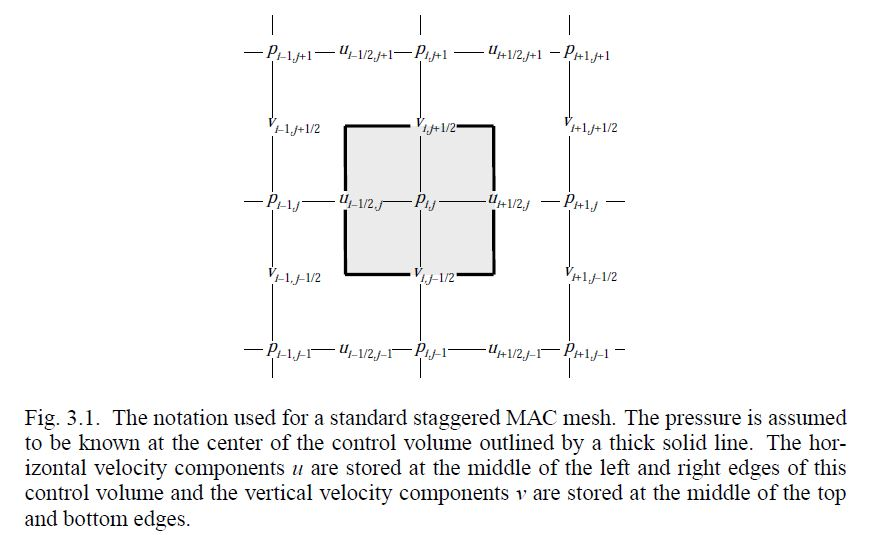
\includegraphics[scale=0.6]{staggered mesh 3.1.JPG}
\centering
\end{figure}
\par
The staggered grid is shown in Fig. 3.1. The starting point is a control volume around the pressure points (outlined by a thick line). The role of pressure for incompressible flows is to force the divergence of the velocity field to be zero: the pressure must be raised if there is a net inflow into this control volume and lowered if there is net outflow. For the computation of the net flow in or out of the control volume around the pressure node we need the horizontal velocity components $u$ at the vertical boundaries and the vertical velocity components $v$ on the horizontal boundaries. It is natural to locate the velocity components at the middle of the boundaries, where we need them, and the grid for the horizontal velocity is therefore displaced half a mesh to the right from the pressure node and the vertical velocity grid is displaced half a mesh upward as shown in Fig.3.2.
\begin{figure}[h]
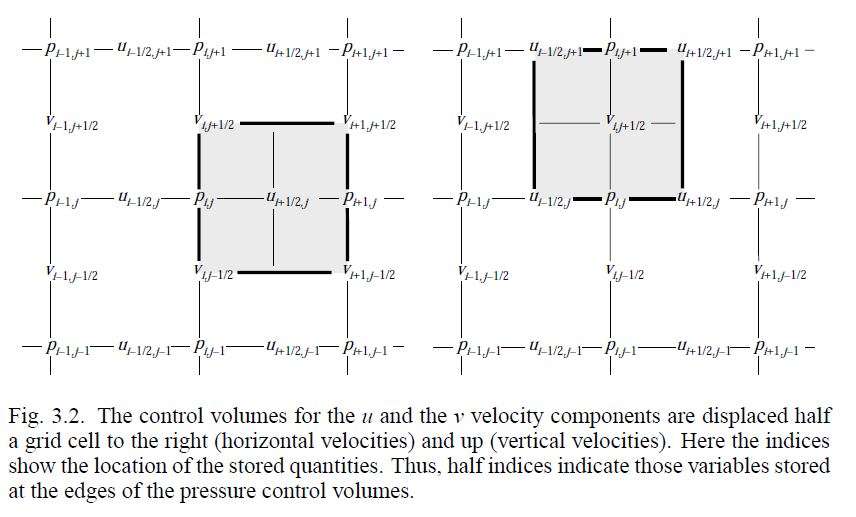
\includegraphics[scale=0.6]{staggered mesh 3.2.JPG}
\centering
\end{figure}
\par
It is customary to identify the pressure nodes by the indices $(i, j)$ and to refer the location of the $u$-velocity component by $(i+1, j)$ and the location of the $v$-velocity component by $(i, j+1)$. \par
On the staggered grid Fig. 3.1, the discrete form of the continuity equation is obtained by writing the integral in Eq(23) for each side of the control volume:
\begin{equation}
\begin{aligned}
0 &=\frac{1}{\Delta x\Delta y} \oint_{S} \textbf{u}^{n+1} \cdot \textbf{n} ds \\ 
&= \frac{1}{\Delta x\Delta y} \left\{
\int_{i+1/2, j} u^{n+1}dy -\int_{i-1/2, j} u^{n+1}dy+\int_{i, j+1/2} v^{n+1}dx-\int_{i, j-1/2} v^{n+1}dx
 \right\}
\end{aligned}
\end{equation}\par
Then by approximating the integrals by the midpoint rule, we have:
\begin{equation}
\frac{1}{\Delta x\Delta y} \left[\left(u_{i+1/2, j}^{n+1}-u_{i-1/2, j}^{n+1}\right)\Delta y +\left(v_{i, j+1/2}^{n+1}-v_{i, j-1/2}^{n+1}\right)\Delta x\right] = 0
\end{equation}\par
Rewriting the equation we can get:
\begin{equation}
\frac{u_{i+1/2, j}^{n+1}-u_{i-1/2, j}^{n+1}}{\Delta x}+\frac{v_{i, j+1/2}^{n+1}-v_{i, j-1/2}^{n+1}}{\Delta y} = 0
\end{equation}\par
\begin{figure}[h]
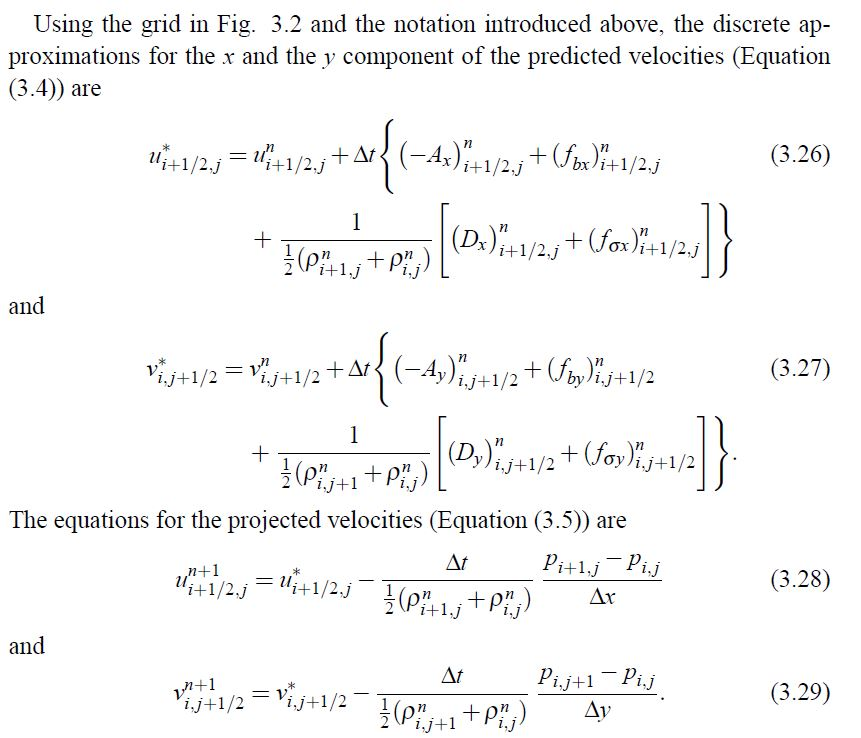
\includegraphics[scale=0.6]{Predicted velocity.JPG}
\centering
\end{figure}\par
There are three main reason why the staggered grid is so widely used  instead of collocated grid where all the variables are located at the same point. One is accuracy. Since the pressure gradient is computed as the difference between adjacent point, versus points two $\Delta x$ or $\Delta y$ apart when a collocated grid is used, the mesh is in effect finer. The second reason is that it is relatively simple to preduce conservative methods when working on a staggered grid. The third is that it results in a tighter coupling between the variables than if they were all located at the same grid node. 
\vspace{3mm}
\textbf{Discretization of the advection terms}\par
The discrete approximation of the $x$-component of the advection term is found by approximating the integral in Eq(19) by the midpoint rule:
$$
\textbf{A}_{c} = \frac{1}{V}  \int_{V} \nabla \cdot (\textbf{uu})dv=\frac{1}{V}  \oint_{S}  (\textbf{uu}) \cdot \textbf{n}ds = \frac{1}{V}  \oint_{S}  \textbf{u}(\textbf{u} \cdot \textbf{n})ds
$$in the 2D case, we have $\textbf{u} = (u, v)$ and the normal vector is $(0, 1), (1, 0), (0, -1), (-1, 0)$.\\
The difference between the left and right side is $u (u,v)\cdot(1,0)$+$u (u,v)\cdot(-1,0)$\\
The difference between the top and bottom side is $u (u,v)\cdot(0,1)$+$u (u,v)\cdot(0,-1)$\\
\begin{equation}
(A_{x})_{i+1/2, j} = \frac{1}{\Delta x\Delta y} \left\{\left[
(uu)_{i+1, j} -(uu)_{i, j}\right] \Delta y +\left[ (uv)_{i+1/2, j+1/2} -(uv)_{i+1/2, j-1/2}\right]\Delta x
\right\}
\end{equation}
Here the advection term is corresponding to certain velocity $(A_{x})_{i+1/2, j} \to u_{i+1/2, j}$ as shown in Fig. 3.2. The this explain why the left side is $(uu)_{i, j}$ and the right side is $(uu)_{i+1, j}$, the top side is $(uv)_{i+1/2, j+1/2}$  and the bottom side is $(uv)_{i+1/2, j-1/2}$. 
\begin{figure}[h]
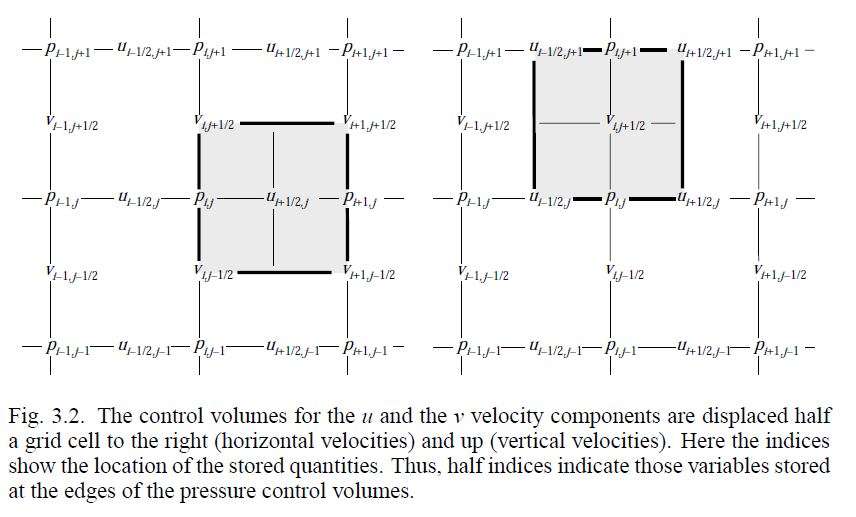
\includegraphics[scale=0.6]{staggered mesh 3.2.JPG}
\centering
\end{figure}\par 
The y-component is approximateed as:
\begin{equation}
(A_{y})_{i, j+1/2} = \frac{1}{\Delta x\Delta y} \left\{\left[
(uv)_{i+1/2, j+1/2} -(uv)_{i-1/2, j+1/2}\right] \Delta y +\left[ (vv)_{i, j+1} -(vv)_{i, j}\right]\Delta x
\right\}
\end{equation}


























\end{document}



























